\documentclass{article}
\usepackage{amsmath}
\usepackage{graphicx}

\begin{document}
\title{Everything}
\author{Logan Bontrager}
\maketitle


\section*{Introduction}

The intent of the project was to explore bayesian time series analysis through autoregressive models. Autoregressive models or AR were introduced in the 1980's to capture casual relationships between macroeconomic variables and have since progressed to be an industry benchmark for time series analysis. The following explores autoregressive models and their bayesian counterparts. Note that for this project, all time series model are self-implemented while all statistical tests are sourced from the statsmodel python package.

\section*{Autoregression}

The autoregressive model assumes that there is a relationship between a vector of observations and a given number of lagged data points. Thus, the model formulates the current times series values as a linear combination of $p$ past observations. This is given by

\[y_t = \beta_0 + \beta_1 y_{t-1} + ... + \beta_{t-p} y_{t-p} + u_t\]
where $\beta$ is the weight vector, $Y = (y_t, y_{t-1}, ..., y_1)$ represents the vector of observations, and $U$ is the error vector.

\section*{Bayesian Autoregression}

For the Bayesian approach, I augmented the model using a simple prior, $\beta \sim N(0, \frac{1}{\alpha}I)$, and learned the parameters for the posterior distribution using the evidence approximation and the iterative algorithm from the book (eq. 3.91, 3.92, and 3.95). Then, we can use these values to find predictions for unobserved values with the maximum a posterior and compute an error value.

\section*{Implementation}

For this project, I will be modeling from the original FANG stock group, Facebook, Amazon, Netflix, and Google. I sourced my data from the Alpha Vantage API. This report will only cover the Amazon ticker in sake of conciseness. The series themselves consist of daily closing price for each respective stock from the last 8 years. 
\\ \\
An important concept in time series analysis with the VAR model is stationarity. Stationarity in academic litature is divided into weak and strict stationarity. For our context, we will be using weak stationarity, or the case where a time series's mean, variance, and correlation doesn't vary with time. Strict stationarity refers to when the joint distribution of observations is consistent over time.
\\ \\
A common test used to check for time series stationarity is the Augmented Dickey Fuller test, ADF. The test assesses the pressence of a unit root in the data or a stochastic trend that could lead us to believe that the underlying distribution is not consistent over time. ADF is given by,

\[y_t = c + \beta t + \alpha y_{t-1} + \phi_1 \Delta Y_{t-2} + ... + \phi_p \Delta Y_{t-p} + u_t\]
In addition, we also need to do exploratory analysis on the series autocorrelation or correlation of the series with itself. This will allow us to determine if the data has seasonality and give us insight into how to properly transform it for the model. The autocorrelation and partial aurocorrelation function are described below for times $s$ and $t$.
\[ACF_x(s,t)=cov(x_s,x_t)=E[(x_s-\mu_s)(x_t-\mu_t)]\]
\[PACF_x(s,t)=\frac{cov(x_s,x_{s-t}|x_{s-1}, ..., x_{s-t+1})}{\sqrt{var(x_s|x_{s-1}, ..., x_{s-t+1})var(x_{s-t}|x_{s-1}, ..., x_{s-t+1})}}\]
These tests will allow us to determine the conditional and non-conditional correlation of a given data point and higher order lags.
\\ \\
The initial results for the raw AMZN data for the ADF test, ACF, and PACF are below.
\\
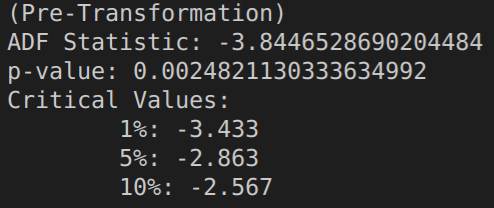
\includegraphics[width=0.6\textwidth]{../output/pre-adf.png}

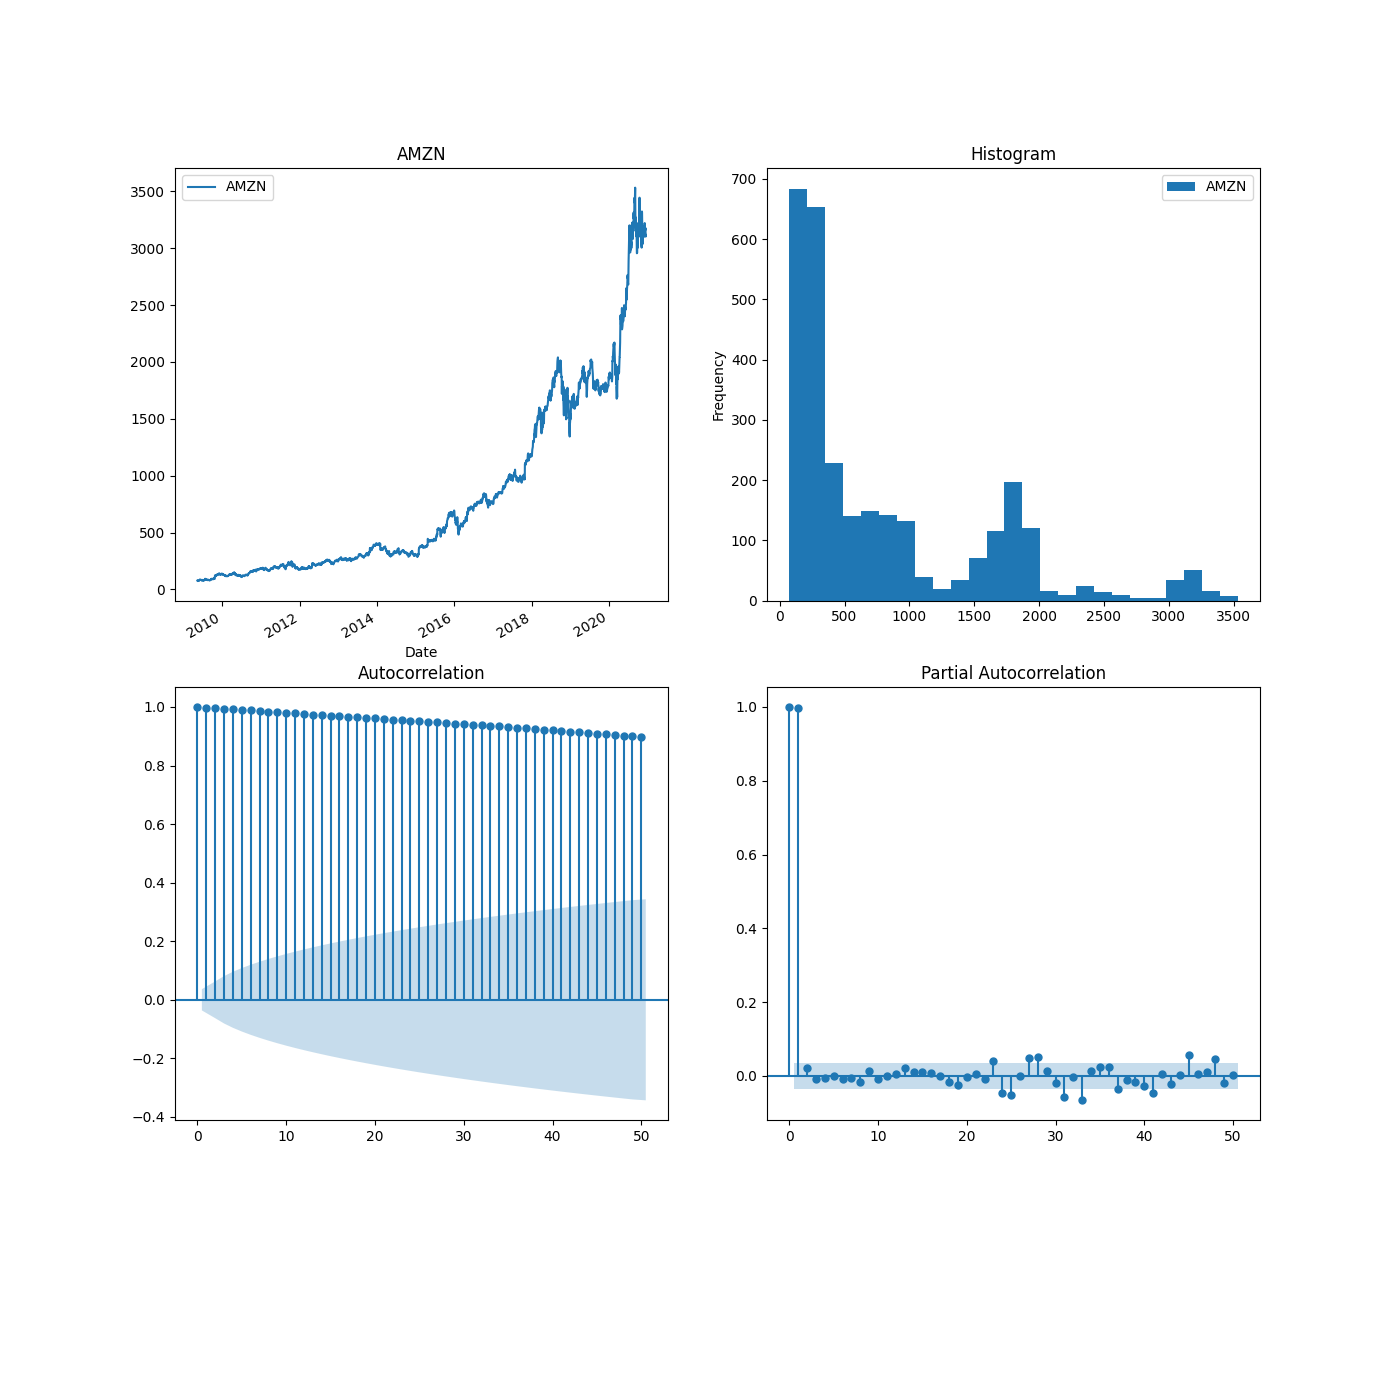
\includegraphics[width=\textwidth]{../output/AMZN_summary.png}
Here, we actually see that our time series passes the ADF test if we assume a $p$ value tolerance of 0.05. Although, we also see a strong correlation with the first conditionally lagged variable and and see that the autocorrelation of the series decreases rather slowly. From the plotted series, it is apparent that the series has a significant trend but no seasonality. Given all this information, we can use first differencing to remove the trend. The exact mathematically operation is $y_t = \log(\frac{y_t}{y_{t-1}})$. The updated summary plots are below. We can see that the autocorrelation both conditional and non-conditional are significantly decreased. Thus, it will be much easier to model the series as a linear combination of past value given our assumptions.

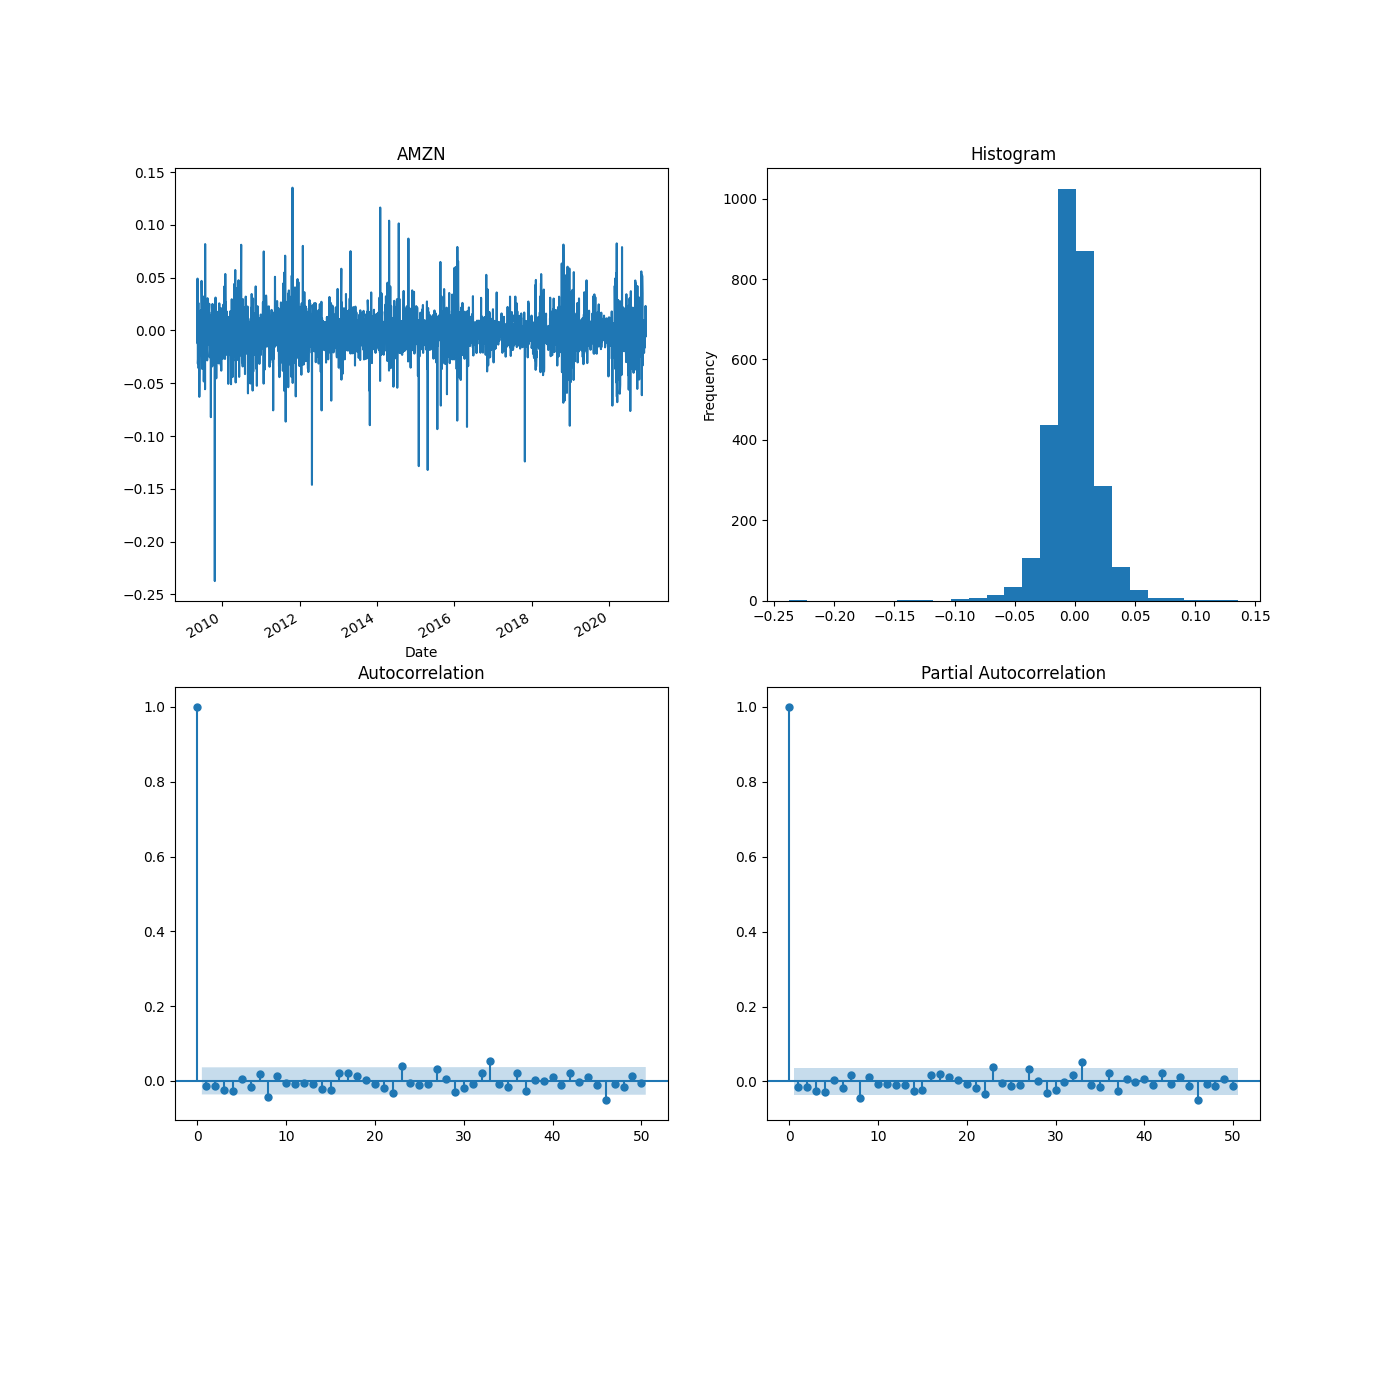
\includegraphics[width=\textwidth]{../output/AMZN_trans_summary.png}

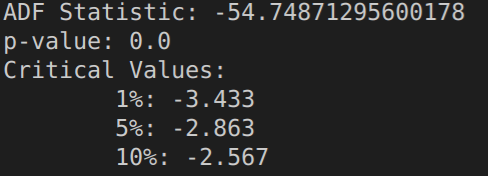
\includegraphics[width=0.6\textwidth]{../output/post-adf.png}

\section*{Lag \& Training Size Tests}

For the following, I used 30 averaged trials (given random row sampling) to compute the respective mean squared error value on the differenced data. From the partial autocorrelation analysis above, we know that the model is likely to perform best when using a single lagged variable. The following graph justifies this belief. We see that as we increase the lag used in the model the error increases. Something that is interesting to note is that the BAR model performs better than the autoregressive model as lags increase.
\\
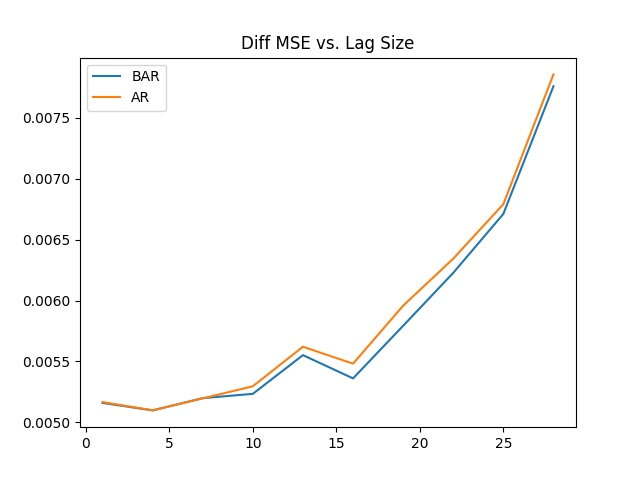
\includegraphics[width=\textwidth]{../output/AMZN_lag_size.png}
\\
The following is the mean squared error of the bayesian and autoregressive model on various training sizes of data which were sampled randomly. It is apparent that the bayesian model performs quite well across all training sizes while the autoregressive model improves drastically as the training percentage increases but does not quite converge to its bayesian counterpart. This is likely due to the mean centered prior which helps bring the predictions towards the data's first moment.

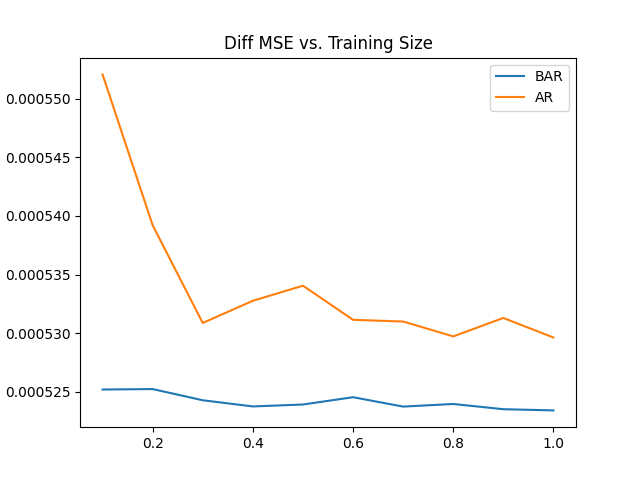
\includegraphics[width=\textwidth]{../output/AMZN_training_size.png}


\section*{Post Discussion}

Initially, I wanted to explore the multivariate VAR  and BSTS model with more complex priors but found myself gravitating towards the autoregressive model when I had issues implementing high dimensional matrix operations. This was a major bottleneck for me. Despite, I believe I got a solid introduction to time series analysis and many of the tips and tricks used for exploring relevant data. If I were to redo the project, I would definitely have spent my time wiser and pursued a more directed goal rather than trying to implement multiple models simultaneously.

\section*{Code Archive}

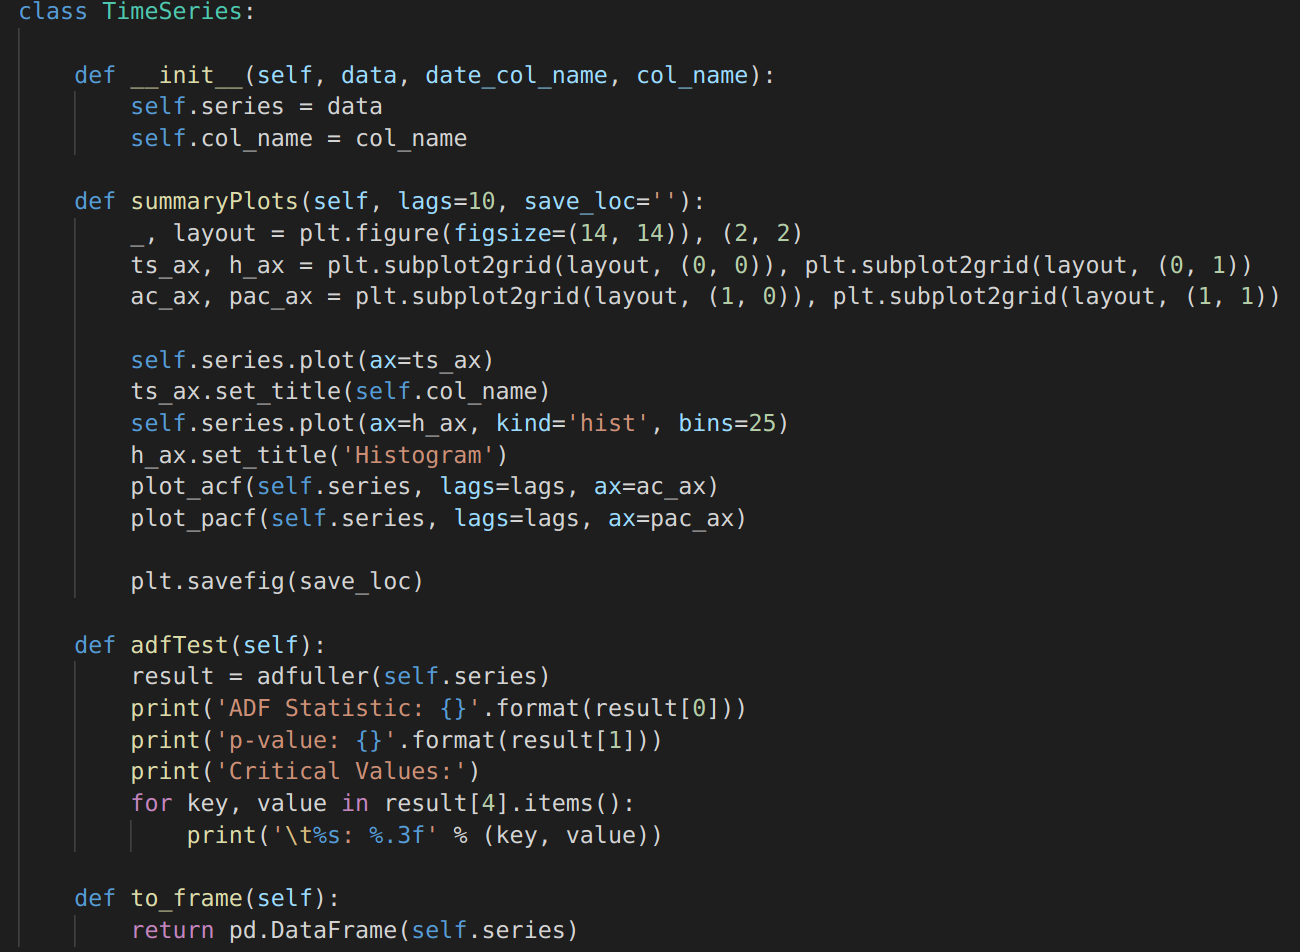
\includegraphics[width=\textwidth]{../output/code2.png}

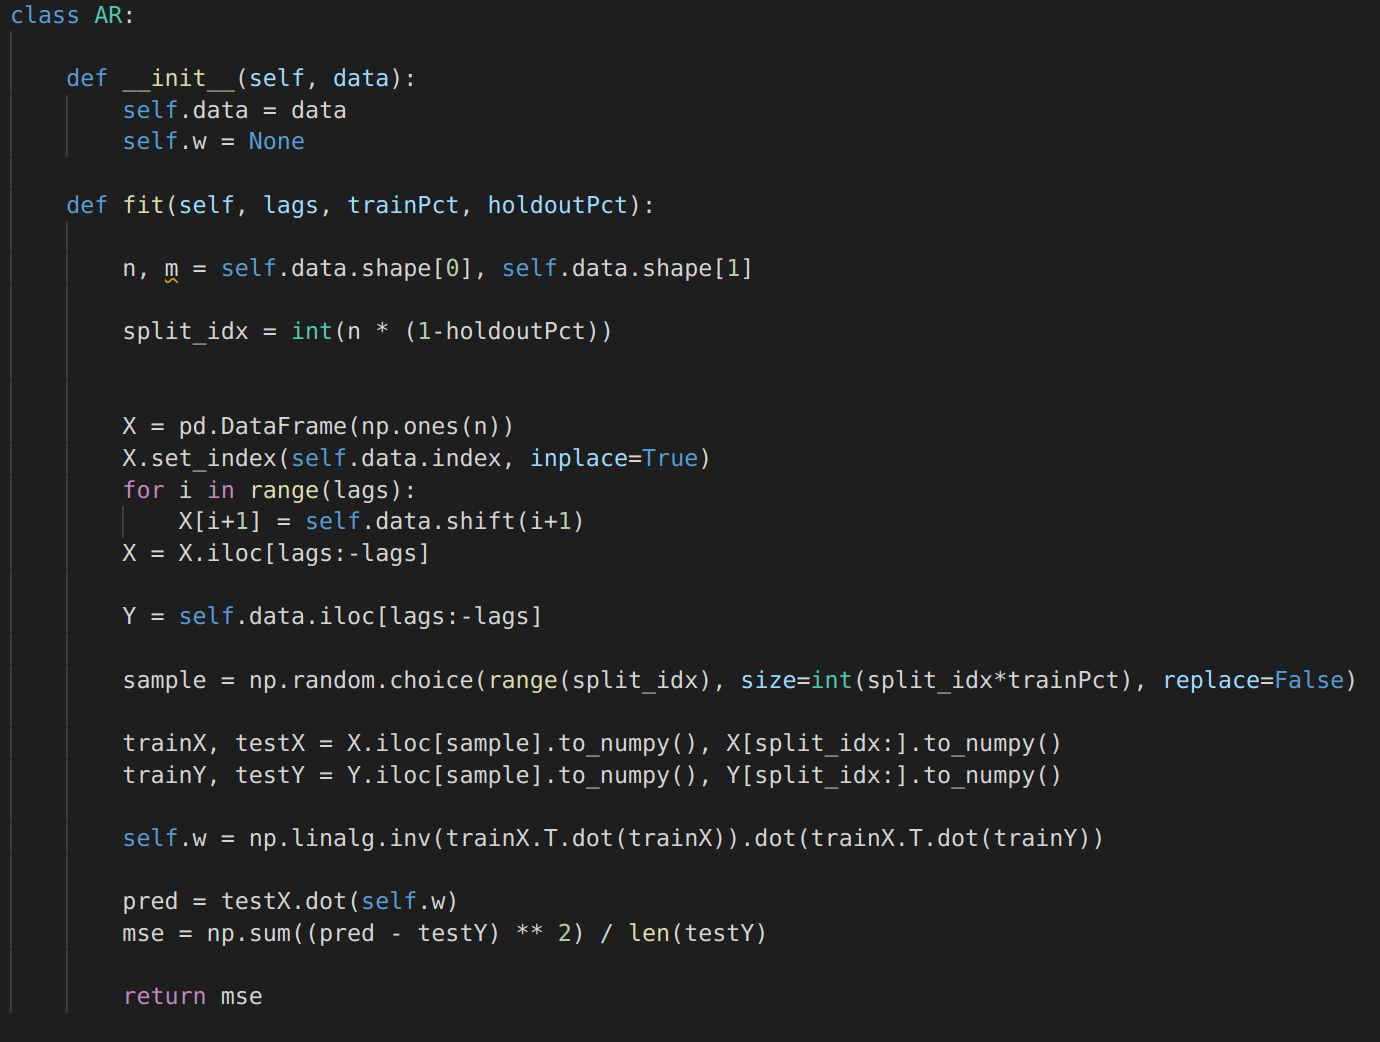
\includegraphics[width=\textwidth]{../output/code3.png}

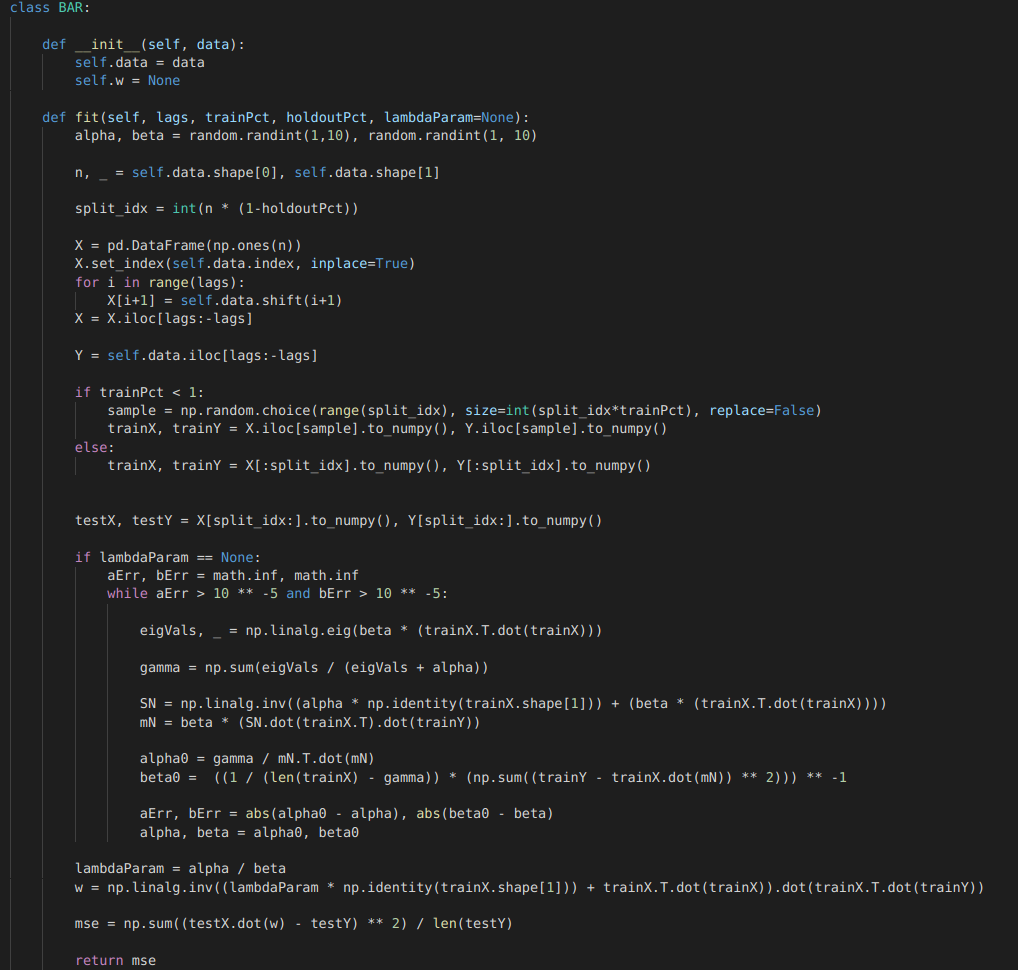
\includegraphics[width=\textwidth]{../output/code1.png}
\end{document}
